\chapter{Discrete Exterior Calculus}
\label{ch:discrete_exterior}

\section{Hodge Star Computation}
\label{sec:hodge_star}

\subsection{Overview}
The \index{Hodge star}Hodge star operator ($*$) is a fundamental tool in \index{Riemannian geometry}Riemannian geometry and \index{exterior calculus}exterior calculus that establishes a correspondence between $k$-forms and $(n-k)$-forms. In \index{discrete exterior calculus}Discrete Exterior Calculus (DEC)~\cite{desbrun2005,crane2013}, the Hodge star operator is represented as a diagonal matrix that maps discrete forms on a primal mesh to discrete forms on its dual mesh. It is essential for solving \index{partial differential equations}partial differential equations (PDEs), such as the \index{Poisson equation}Poisson equation or Maxwell's equations, on triangle meshes.

\subsection{Definitions}
\begin{definition}[Discrete $k$-Form]\label{def:discrete_k_form}
A scalar value associated with each $k$-simplex of a mesh (0-form: vertex, 1-form: edge, 2-form: face). More precisely, a discrete $k$-form is an element of the dual space $\Omega^k(K) = C^k(K; \mathbb{R})$, where $C^k$ is the space of $k$-\index{cochain}cochains on the simplicial complex $K$.
\end{definition}

\begin{definition}[Primal Mesh]\label{def:primal_mesh}
The original triangular mesh, consisting of vertices ($V$), edges ($E$), and faces ($F$). The \index{primal mesh}primal mesh serves as the domain on which discrete differential operators are defined.
\end{definition}

\begin{definition}[Dual Mesh]\label{def:dual_mesh}
Typically the Voronoi diagram or the \index{circumcentric dual}circumcentric dual of the primal mesh. Each primal $k$-simplex corresponds to a dual $(n-k)$-simplex, establishing a bijection between the primal and dual cell complexes.
\end{definition}

\begin{definition}[Hodge Star ($\star$)]\label{def:hodge_star}
An operator that maps a discrete form on a primal simplex to its dual simplex, preserving ``flow'' or ``intensity'' across the two. The Hodge star $\star_k \colon \Omega^k(K) \to \Omega^{n-k}(K^\star)$ encodes the local metric information of the mesh.
\end{definition}

\subsection{Theory}
In 2D (surface meshes), the discrete Hodge star operators are typically defined as follows:
\begin{itemize}
    \item \textbf{0-star ($\star_0$)}: Maps a value at a primal vertex to its dual Voronoi cell. $\star_0 = \frac{\text{Area(Dual Cell)}}{\text{Area(Primal Vertex)}} = \text{Area(Dual Cell)}$.
    \item \textbf{1-star ($\star_1$)}: Maps a value on a primal edge to its dual Voronoi edge. $\star_1 = \frac{\text{Length(Dual Edge)}}{\text{Length(Primal Edge)}}$. This is the famous \index{cotangent weight}cotangent weight ratio: $\frac{1}{2}(\cot \alpha + \cot \beta)$.
    \item \textbf{2-star ($\star_2$)}: Maps a value on a primal face to its dual Voronoi vertex. $\star_2 = \frac{\text{Area(Dual Vertex)}}{\text{Area(Primal Face)}} = \frac{1}{\text{Area(Primal Face)}}$.
\end{itemize}

\begin{theorem}[Cotangent Weight Formula]\label{thm:cotangent_weight}
The discrete 1-Hodge star on a triangulated surface with circumcentric dual is given by the cotangent weights:
\[
(\star_1)_{e} = \frac{1}{2}(\cot \alpha_e + \cot \beta_e),
\]
where $\alpha_e$ and $\beta_e$ are the angles opposite to edge $e$ in the two adjacent triangles. These weights are non-negative if and only if the two triangles sharing edge $e$ form an intrinsic Delaunay triangulation.
\end{theorem}

\begin{proof}
Consider an edge $e = (u,v)$ shared by two triangles $\triangle uvw_1$ and $\triangle uvw_2$. The dual edge $e^\star$ connects the circumcenters $c_1, c_2$ of the two triangles. Since the circumcenter lies at the intersection of perpendicular bisectors, the dual edge $e^\star$ is perpendicular to the primal edge $e$. By elementary trigonometry, the length of the dual edge satisfies
\[
|e^\star| = \frac{1}{2}|e|(\cot \alpha_e + \cot \beta_e),
\]
where $\alpha_e = \angle uw_1v$ and $\beta_e = \angle uw_2v$. Dividing by $|e|$ yields the stated ratio. The non-negativity condition follows from the fact that $\cot \theta > 0$ for $\theta < \pi/2$ and $\cot \theta < 0$ for $\theta > \pi/2$~\cite{pinkall1993}.
\end{proof}

\begin{example}[Cotangent Weight on an Equilateral Triangle]\label{ex:cotangent_weight}
Consider two equilateral triangles sharing an edge, forming a rhombus. Each opposite angle is $60^\circ$, so the cotangent weight is:
\[
(\star_1)_e = \frac{1}{2}(\cot 60^\circ + \cot 60^\circ) = \frac{1}{2}\left(\frac{1}{\sqrt{3}} + \frac{1}{\sqrt{3}}\right) = \frac{1}{\sqrt{3}} \approx 0.577.
\]
This is the canonical value for a regular triangulation, and the resulting \index{Laplace-Beltrami operator}Laplacian matrix reduces to the standard 5-point stencil on a regular grid.
\end{example}

These operators allow for the definition of the Discrete Laplace-Beltrami Operator as $\Delta = \star_0^{-1} d^\top \star_1 d$, where $d$ is the discrete exterior derivative~\cite{crane2013}.

\subsection{Pseudocode}
\begin{algorithm}
\caption{Compute Hodge Star Operators}\label{alg:compute_hodge_stars}
\begin{algorithmic}
\Function{ComputeHodgeStars}{mesh}
    \Comment{1. 0-Star (Vertex areas)}
    \State $star0 \gets \text{DiagonalMatrix}(n\_vertices)$
    \ForAll{$v \in \text{mesh.vertices}$}
        \State $star0[v, v] \gets \text{ComputeVoronoiArea}(v, mesh)$
    \EndFor

    \Comment{2. 1-Star (Edge cotangent weights)}
    \State $star1 \gets \text{DiagonalMatrix}(n\_edges)$
    \ForAll{$edge \in \text{mesh.edges}$}
        \State $\alpha, \beta \gets \text{GetOppositeAngles}(edge, mesh)$
        \State $star1[edge, edge] \gets 0.5 \cdot (\cot(\alpha) + \cot(\beta))$
    \EndFor

    \Comment{3. 2-Star (Face areas)}
    \State $star2 \gets \text{DiagonalMatrix}(n\_faces)$
    \ForAll{$face \in \text{mesh.faces}$}
        \State $star2[face, face] \gets 1.0 \;/\; \text{ComputeFaceArea}(face, mesh)$
    \EndFor

    \Return $star0, star1, star2$
\EndFunction
\end{algorithmic}
\end{algorithm}
\Cref{alg:compute_hodge_stars} computes all three diagonal Hodge star matrices in a single pass over the mesh elements. The dominant cost is the Voronoi area and angle computations per element.

\subsection{Parameter Selection}
\begin{itemize}
    \item \textbf{Dual Mesh Choice}: The \textbf{Circumcentric Dual} is preferred because primal edges are perpendicular to dual edges, simplifying the star operator to a simple ratio.
    \item \textbf{Robustness}: Cotangent weights can become negative if the mesh contains obtuse triangles. Using an intrinsic Delaunay triangulation or an epsilon-clamping can mitigate this~\cite{pinkall1993}.
\end{itemize}

\subsection{Complexity}
\begin{itemize}
    \item \textbf{Time Complexity}: $O(F)$, where $F$ is the number of faces, to calculate all local geometric properties (areas, lengths, angles).
    \item \textbf{Space Complexity}: $O(V + E + F)$ to store the diagonal matrices.
\end{itemize}

\subsection{Usages}
\begin{itemize}
    \item \textbf{Surface Parameterization}: Constructing the Laplacian matrix for Harmonic Mapping or LSCM.
    \item \textbf{Mesh Smoothing}: Implementing Mean Curvature Flow using the DEC Laplacian.
    \item \textbf{Fluid Simulation on Surfaces}: Solving the Navier-Stokes equations using discrete forms.
    \item \textbf{Geodesic Distances}: Implementing the Heat Method for distance calculation.
    \item \textbf{Texture Synthesis}: Generating procedural textures by solving reaction-diffusion equations on meshes.
\end{itemize}

\subsection{Testing Methods and Edge Cases}
\begin{itemize}
    \item \textbf{Flat Plane}: On a regular grid, the cotangent weights should simplify to the standard 5-point Laplacian stencil.
    \item \textbf{Equilateral Triangles}: All cotangent weights should be exactly $\cot(60^\circ) = 1/\sqrt{3}$.
    \item \textbf{Obtuse Triangles}: Verify that negative cotangent weights are handled or expected (they can cause instability in some solvers).
    \item \textbf{Boundaries}: Vertices and edges on the boundary have only one incident face; their Hodge star contributions must be halved or handled carefully.
\end{itemize}

\subsection{References}
\begin{itemize}
    \item Desbrun, M., Hirani, A. N., Leok, M., \& Marsden, J. E. (2005). ``Discrete Exterior Calculus''. arXiv preprint.
    \item Crane, K., Weischedel, C., \& Wardetzky, M. (2013). ``Digital Geometry Processing with Discrete Exterior Calculus''. SIGGRAPH Course.
    \item Pinkall, U., \& Polthier, K. (1993). ``Computing discrete minimal surfaces and their conjugates''. Computing.
    \item Wikipedia: Discrete exterior calculus
\end{itemize}


\section{Exterior Derivative}
\label{sec:exterior_derivative}

\subsection{Overview}
The \index{exterior derivative}exterior derivative ($d$) is a fundamental operator in \index{differential geometry}differential geometry that generalizes the concepts of \index{gradient}gradient, \index{curl}curl, and \index{divergence}divergence to higher-dimensional forms. In Discrete Exterior Calculus (DEC)~\cite{desbrun2005,crane2013}, the exterior derivative is a sparse matrix that acts as a topological operator, mapping discrete $k$-forms on a mesh to discrete $(k+1)$-forms. It depends purely on the connectivity of the mesh (its boundary relationships) and is independent of the mesh's geometric coordinates.

\subsection{Definitions}
\begin{definition}[Discrete $k$-Form ($\omega^k$)]\label{def:ext_k_form}
A vector of scalar values, where each entry is associated with a $k$-simplex of the mesh (0-simplex: vertex, 1-simplex: edge, 2-simplex: face). The space of all discrete $k$-forms is denoted $\Omega^k$.
\end{definition}

\begin{definition}[Chain Complex]\label{def:chain_complex}
A sequence of vector spaces of $k$-chains connected by \index{boundary operator}boundary operators ($\partial$):
\[
\cdots \xrightarrow{\partial_{k+1}} C_k \xrightarrow{\partial_k} C_{k-1} \xrightarrow{\partial_{k-1}} \cdots
\]
satisfying the fundamental property $\partial_{k} \circ \partial_{k+1} = 0$ for all $k$.
\end{definition}

\begin{definition}[Cochain Complex]\label{def:cochain_complex}
A sequence of vector spaces of $k$-forms connected by exterior derivatives ($d$):
\[
\cdots \xrightarrow{d_{k-1}} \Omega^k \xrightarrow{d_k} \Omega^{k+1} \xrightarrow{d_{k+1}} \cdots
\]
The cochain complex is dual to the chain complex, and the exterior derivative $d_k$ is the transpose of the boundary operator $\partial_{k+1}$.
\end{definition}

\begin{definition}[Boundary Relationship ($\partial$)]\label{def:boundary_relationship}
The boundary of a 1-simplex (edge) is its two 0-simplices (vertices). The boundary of a 2-simplex (triangle) is its three 1-simplices (edges). More generally, $\partial_k$ maps each $k$-simplex to a formal sum of its $(k-1)$-faces with appropriate orientations.
\end{definition}

\subsection{Theory}
The discrete exterior derivative $d_k$ is the \textbf{dual of the boundary operator} $\partial_{k+1}$ from the primal mesh. Specifically, it maps a value on a $k$-simplex to its incident $(k+1)$-simplices based on orientation.
\begin{itemize}
    \item \textbf{0-derivative ($d_0$)}: Maps a value at vertices to its incident edges. $d_0(\phi)_{(u,v)} = \phi_v - \phi_u$. This is the discrete equivalent of the \textbf{Gradient}.
    \item \textbf{1-derivative ($d_1$)}: Maps a value on edges to its incident faces. $d_1(\alpha)_{(u,v,w)} = \alpha_{uv} + \alpha_{vw} + \alpha_{wu}$ (where indices are oriented). This is the discrete equivalent of the \textbf{Curl}.
\end{itemize}

\begin{theorem}[Null Property of the Exterior Derivative]\label{thm:d_squared_zero}
For any discrete $k$-form $\omega$ on a simplicial complex, the composition $d_{k+1} \circ d_k = 0$. That is, the derivative of a derivative is always zero.
\end{theorem}

\begin{proof}
We verify this directly. Let $\phi$ be a 0-form (vertex values). Then $(d_0 \phi)_{(u,v)} = \phi_v - \phi_u$. Applying $d_1$ to this 1-form yields, for a face $(u,v,w)$:
\[
(d_1 \, d_0 \, \phi)_{(u,v,w)} = (\phi_v - \phi_u) + (\phi_w - \phi_v) + (\phi_u - \phi_w) = 0.
\]
This holds for every face, so $d_1 \, d_0 = 0$ as a matrix product. In higher dimensions, the argument is analogous: each $(k+2)$-simplex has exactly two $(k+1)$-faces that contain each $k$-face, and their contributions cancel due to opposite orientations. This is the discrete version of the identities $\nabla \times (\nabla \phi) = 0$ and $\nabla \cdot (\nabla \times A) = 0$~\cite{desbrun2005}.
\end{proof}

\begin{example}[Exterior Derivative on a Single Triangle]\label{ex:exterior_derivative_triangle}
Let a triangle have vertices $u, v, w$ with a 0-form $\phi(u) = 1$, $\phi(v) = 3$, $\phi(w) = 0$. The 1-form $d_0 \phi$ assigns values to oriented edges:
\[
(d_0 \phi)_{uv} = 3 - 1 = 2, \quad (d_0 \phi)_{vw} = 0 - 3 = -3, \quad (d_0 \phi)_{wu} = 1 - 0 = 1.
\]
Applying $d_1$:
\[
(d_1 \, d_0 \, \phi)_{uvw} = 2 + (-3) + 1 = 0,
\]
confirming the null property $d_1 \circ d_0 = 0$.
\end{example}

\begin{figure}[htbp]
\centering
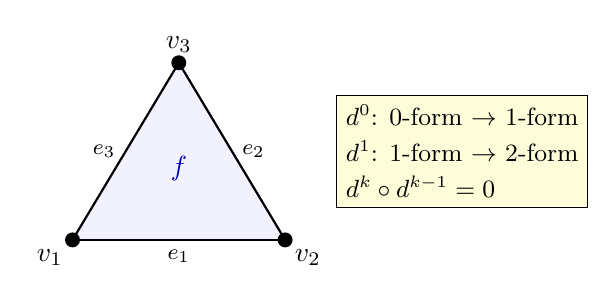
\begin{tikzpicture}[scale=0.9]
  \coordinate (v1) at (0,0);
  \coordinate (v2) at (3,0);
  \coordinate (v3) at (1.5,2.5);
  \fill[blue!5] (v1)--(v2)--(v3)--cycle;
  \draw[thick] (v1)--(v2) node[midway,below,font=\footnotesize] {$e_1$};
  \draw[thick] (v2)--(v3) node[midway,right,font=\footnotesize] {$e_2$};
  \draw[thick] (v3)--(v1) node[midway,left,font=\footnotesize] {$e_3$};
  \fill (v1) circle (3pt) node[below left] {$v_1$};
  \fill (v2) circle (3pt) node[below right] {$v_2$};
  \fill (v3) circle (3pt) node[above] {$v_3$};
  \node[blue!70!black] at (1.5,1) {$f$};
  \node[draw,rectangle,fill=yellow!15,font=\small,align=left] at (5.5,1.25) {
    $d^0$: 0-form $\to$ 1-form\\[2pt]
    $d^1$: 1-form $\to$ 2-form\\[2pt]
    $d^k \circ d^{k-1} = 0$
  };
\end{tikzpicture}
\caption{Discrete exterior derivative: $d^0$ maps vertex values to edge differences; $d^1$ maps edge values to face circulations.}
\label{fig:exterior_derivative}
\end{figure}


\subsection{Pseudocode}
\begin{algorithm}
\caption{Compute Exterior Derivatives}\label{alg:compute_exterior_derivatives}
\begin{algorithmic}
\Function{ComputeExteriorDerivatives}{mesh}
    \Comment{1. d0 (0-forms to 1-forms)}
    \State $d0 \gets \text{SparseMatrix}(n\_edges, n\_vertices)$
    \ForAll{$edge \in \text{mesh.edges}$}
        \State $u, v \gets edge.start\_vertex, edge.end\_vertex$
        \State $d0[edge\_id, v] \gets 1$
        \State $d0[edge\_id, u] \gets -1$
    \EndFor

    \Comment{2. d1 (1-forms to 2-forms)}
    \State $d1 \gets \text{SparseMatrix}(n\_faces, n\_edges)$
    \ForAll{$face \in \text{mesh.faces}$}
        \ForAll{$(edge\_id, orientation) \in \text{GetOrientedEdges}(face)$}
            \State $d1[face\_id, edge\_id] \gets orientation$
        \EndFor
    \EndFor

    \Return $d0, d1$
\EndFunction
\end{algorithmic}
\end{algorithm}
Note that \Cref{alg:compute_exterior_derivatives} requires only the mesh connectivity (vertex-edge and edge-face incidence), not any geometric information such as vertex positions or edge lengths.

\subsection{Parameter Selection}
\begin{itemize}
    \item \textbf{Orientation}: All simplices must be consistently oriented. Primal edges are typically oriented by vertex ID (e.g., $u \to v$ if $u < v$). Primal faces are usually CCW.
    \item \textbf{Sparse Representation}: Since each simplex has only a few neighbors, $d$ matrices are extremely sparse; CSR or CSC formats are essential for performance.
\end{itemize}

\subsection{Complexity}
\begin{itemize}
    \item \textbf{Time Complexity}: $O(F)$, where $F$ is the number of faces, as we iterate through each face and edge relationship once.
    \item \textbf{Space Complexity}: $O(E + F)$ to store the sparse matrix entries.
\end{itemize}

\subsection{Usages}
\begin{itemize}
    \item \textbf{Vector Field Processing}: Decomposing vector fields into curl-free and divergence-free components (\index{Hodge decomposition}Hodge Decomposition).
    \item \textbf{Surface Parameterization}: Representing gradients of scalar functions used in UV mapping.
    \item \textbf{Fluid Simulation}: Enforcing divergence-free conditions on flow velocities.
    \item \textbf{Solving PDEs}: Formulating the Poisson or Heat equation using the DEC Laplacian $\Delta = \star^{-1} d^\top \star d$.
    \item \textbf{Topology Analysis}: Computing \index{Betti number}Betti numbers or identifying mesh ``holes'' using \index{homology}homology.
\end{itemize}

\subsection{Testing Methods and Edge Cases}
\begin{itemize}
    \item \textbf{d o d Property}: Verify that $d_1 \times d_0$ results in a matrix where all entries are near zero (floating point) or exactly zero (integer).
    \item \textbf{Single Triangle}: On a single triangle, the sum of edge values around the boundary must match the face derivative.
    \item \textbf{Disconnected Mesh}: The matrices should naturally decompose into block-diagonal structures for each component.
    \item \textbf{Boundaries}: Ensure that orientation is handled correctly for edges on the mesh boundary.
\end{itemize}

\subsection{References}
\begin{itemize}
    \item Desbrun, M., Hirani, A. N., Leok, M., \& Marsden, J. E. (2005). ``Discrete Exterior Calculus''. arXiv preprint.
    \item Crane, K., Weischedel, C., \& Wardetzky, M. (2013). ``Digital Geometry Processing with Discrete Exterior Calculus''. SIGGRAPH Course.
    \item Wikipedia: Exterior derivative
\end{itemize}


\section{Hodge Decomposition}
\label{sec:hodge_decomposition}

\subsection{Overview}
The Hodge-Helmholtz Decomposition (often simply \index{Hodge decomposition}Hodge Decomposition) is a fundamental theorem in vector calculus and differential geometry that states any vector field can be uniquely decomposed into three orthogonal components: a \index{curl-free}curl-free component (the gradient of a scalar potential), a \index{divergence-free}divergence-free component (the curl of a vector potential), and a \index{harmonic component}harmonic component (representing flow around topological ``holes''). In the context of 2D surface meshes, it provides a powerful way to analyze and manipulate tangent vector fields~\cite{crane2013,tong2003}.

\subsection{Definitions}
\begin{definition}[Exact Component ($\omega_{\text{exact}}$)]\label{def:exact_component}
The gradient of a scalar function $\alpha$, $\omega_{\text{exact}} = d\alpha$. These are \textbf{curl-free}, meaning $d(\omega_{\text{exact}}) = d(d\alpha) = 0$ by \cref{thm:d_squared_zero}. In $\mathbb{R}^3$ notation, $\omega_{\text{exact}} = \nabla \alpha$.
\end{definition}

\begin{definition}[Co-exact Component ($\omega_{\text{co-exact}}$)]\label{def:coexact_component}
The ``rotational'' part, represented as $\omega_{\text{co-exact}} = \star d\beta$. These are \textbf{divergence-free}, meaning $\delta(\omega_{\text{co-exact}}) = 0$, where $\delta = \star^{-1} d^\top \star$ is the \index{codifferential}codifferential. In $\mathbb{R}^3$ notation, $\omega_{\text{co-exact}} = \nabla \times \mathbf{A}$ for some vector potential $\mathbf{A}$.
\end{definition}

\begin{definition}[Harmonic Component ($\omega_{\text{harmonic}}$)]\label{def:harmonic_component}
A field that is both curl-free and divergence-free, $d\omega = \delta\omega = 0$. These depend on the topology of the mesh---specifically, on the \index{Betti number}Betti numbers of the surface. On a closed surface of genus $g$, there are exactly $2g$ linearly independent harmonic 1-forms~\cite{polthier2003}.
\end{definition}

\subsection{Theory}
In Discrete Exterior Calculus (DEC), the decomposition is performed by solving two separate Poisson equations~\cite{crane2013}:
\begin{enumerate}
    \item \textbf{Gradient Part}: Minimize the energy $\| \omega - d\alpha \|^2$ to find the scalar potential $\alpha$. This leads to the linear system $\Delta \alpha = \delta \omega$, where $\delta = \star^{-1} d^\top \star$ is the codifferential (divergence).
    \item \textbf{Curl Part}: Minimize the energy $\| \omega - \delta\beta \|^2$ to find the dual potential $\beta$. This leads to the linear system $\Delta \beta = d \omega$, where $d$ is the curl.
    \item \textbf{Harmonic Part}: The remainder $\gamma = \omega - d\alpha - \delta\beta$ is the harmonic component.
\end{enumerate}

Orthogonality between these components is guaranteed by the $d \circ d = 0$ property (\cref{thm:d_squared_zero}) and the definition of the Hodge star.

\begin{theorem}[Helmholtz-Hodge Decomposition]\label{thm:hodge_decomposition}
For any 1-form $\omega$ on a compact, oriented Riemannian 2-manifold, there exist unique forms $\alpha$ (0-form), $\beta$ (2-form), and $\gamma$ (harmonic 1-form) such that:
\[
\omega = d\alpha + \star d\beta + \gamma,
\]
where $d\alpha$ is exact (curl-free), $\star d\beta$ is co-exact (divergence-free), and $\gamma$ is harmonic. Moreover, the three components are mutually orthogonal under the $L^2$ inner product:
\[
\langle d\alpha, \star d\beta \rangle = \langle d\alpha, \gamma \rangle = \langle \star d\beta, \gamma \rangle = 0.
\]
\end{theorem}

\begin{proof}
We construct the decomposition explicitly. Given a 1-form $\omega$:

\emph{Step 1 (Exact part):} Solve $\Delta \alpha = \delta \omega$ for $\alpha$, where $\Delta = d^\top \star_1^{-1} d + d_1^\top \star_2 d_1^{-1} \cdots$ is the \index{Laplace-Beltrami operator}discrete Laplacian. Define $\omega_{\text{exact}} = d\alpha$. Then $\delta(\omega - d\alpha) = \delta\omega - \Delta\alpha = 0$.

\emph{Step 2 (Co-exact part):} Solve $\Delta \beta = d(\omega - d\alpha)$ for $\beta$. Define $\omega_{\text{co-exact}} = \star d\beta$. By \cref{thm:d_squared_zero}, $d(\star d\beta) = 0$, so the co-exact part is divergence-free.

\emph{Step 3 (Harmonic part):} Set $\gamma = \omega - d\alpha - \star d\beta$. By construction, $d\gamma = d\omega - d(d\alpha) - d(\star d\beta) = d\omega - 0 - 0 = d\omega - d\omega = 0$, and similarly $\delta\gamma = 0$.

Orthogonality follows from $\langle d\alpha, \star d\beta \rangle = \langle \alpha, d^\top \star d\beta \rangle = \langle \alpha, \Delta \beta \rangle$ and the self-adjointness of $\Delta$~\cite{tong2003}.
\end{proof}

\begin{example}[Hodge Decomposition on a Torus]\label{ex:hodge_decomposition_torus}
Consider a uniform vector field $\omega$ flowing around the major circumference of a torus (genus $g = 1$). Since the field has no local variation, both $d\omega$ and $\delta\omega$ are zero, meaning $\omega$ is itself harmonic: $\omega = \gamma$. The exact and co-exact components are both zero. This demonstrates that harmonic components capture global topological flow---they cannot be expressed as local gradients or curls~\cite{polthier2003}.
\end{example}

\begin{figure}[htbp]
\centering
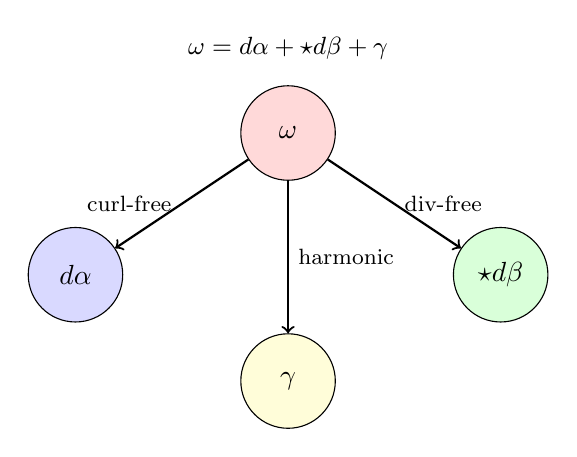
\begin{tikzpicture}[scale=0.9]
  \node[draw,circle,fill=red!15,minimum size=1.2cm] (omega) at (0,0) {$\omega$};
  \node[draw,circle,fill=blue!15,minimum size=1.2cm] (exact) at (-3,-2) {$d\alpha$};
  \node[draw,circle,fill=green!15,minimum size=1.2cm] (coexact) at (3,-2) {$\star d\beta$};
  \node[draw,circle,fill=yellow!15,minimum size=1.2cm] (harmonic) at (0,-3.5) {$\gamma$};
  \draw[->,thick] (omega)--(exact) node[midway,left,font=\footnotesize] {curl-free};
  \draw[->,thick] (omega)--(coexact) node[midway,right,font=\footnotesize] {div-free};
  \draw[->,thick] (omega)--(harmonic) node[midway,right,font=\footnotesize] {harmonic};
  \node[font=\small,align=center] at (0,1.2) {$\omega = d\alpha + \star d\beta + \gamma$};
\end{tikzpicture}
\caption{Hodge decomposition: any 1-form $\omega$ splits uniquely into exact, co-exact, and harmonic components.}
\label{fig:hodge_decomp}
\end{figure}


\subsection{Pseudocode}
\begin{algorithm}
\caption{Hodge Decomposition of a 1-Form}\label{alg:hodge_decompose}
\begin{algorithmic}
\Function{HodgeDecompose}{omega, mesh}
    \Comment{1. Compute discrete operators}
    \State $d0, d1 \gets \text{ComputeExteriorDerivatives}(mesh)$ \Comment{\cref{alg:compute_exterior_derivatives}}
    \State $star0, star1, star2 \gets \text{ComputeHodgeStars}(mesh)$ \Comment{\cref{alg:compute_hodge_stars}}

    \Comment{2. Find Exact Component ($d\alpha$)}
    \State $Laplacian\_0 \gets d0^\top \cdot star1 \cdot d0$
    \State $rhs\_exact \gets d0^\top \cdot star1 \cdot omega$
    \State $\alpha \gets \text{SolveSparse}(Laplacian\_0, rhs\_exact)$
    \State $exact\_part \gets d0 \cdot \alpha$

    \Comment{3. Find Co-exact Component ($\star d\beta$)}
    \State $Laplacian\_1 \gets d1 \cdot star1^{-1} \cdot d1^\top$
    \State $rhs\_coexact \gets d1 \cdot omega$
    \State $\hat{\beta} \gets \text{SolveSparse}(Laplacian\_1, rhs\_coexact)$
    \State $coexact\_part \gets star1^{-1} \cdot d1^\top \star2^{-1} \cdot \hat{\beta}$

    \Comment{4. Harmonic Part}
    \State $harmonic\_part \gets omega - exact\_part - coexact\_part$

    \Return $exact\_part, coexact\_part, harmonic\_part$
\EndFunction
\end{algorithmic}
\end{algorithm}
As shown in \Cref{alg:hodge_decompose}, the algorithm relies on \cref{alg:compute_exterior_derivatives,alg:compute_hodge_stars} as subroutines and requires solving two sparse linear systems.

\subsection{Parameter Selection}
\begin{itemize}
    \item \textbf{Boundary Conditions}: For meshes with boundaries, the decomposition is not unique unless boundary conditions are specified (e.g., $d\alpha$ is normal or tangent to the boundary).
    \item \textbf{Sparse Solver}: Cholesky factorization (via \texttt{scipy.sparse.linalg.factorized}) is recommended as the Laplacian matrices are symmetric and positive semi-definite.
\end{itemize}

\subsection{Complexity}
\begin{itemize}
    \item \textbf{Time Complexity}: $O(E^{1.5})$ where $E$ is the number of edges, dominated by the sparse linear solver performance.
    \item \textbf{Space Complexity}: $O(E)$ to store the discrete operators and the field vectors.
\end{itemize}

\subsection{Usages}
\begin{itemize}
    \item \textbf{Vector Field Design}: Creating smooth vector fields for hair, fur, or pen-and-ink rendering by manipulating the potentials.
    \item \textbf{Surface Parameterization}: Constructing ``conformal'' maps by ensuring the gradient field of UV coordinates is harmonic.
    \item \textbf{Fluid Animation}: Extracting the rotational (co-exact) part of a flow for vortex visualization or removing divergence to maintain volume.
    \item \textbf{Shape Matching}: Using harmonic components as topological signatures for 3D models.
    \item \textbf{Meteorology}: Analyzing global wind patterns into geostrophic (exact) and ageostrophic components.
\end{itemize}

\subsection{Testing Methods and Edge Cases}
\begin{itemize}
    \item \textbf{Pure Gradient Field}: If $\omega = d\phi$ for some random scalar $\phi$, then the co-exact and harmonic parts should be nearly zero.
    \item \textbf{Zero-Genus Mesh}: On a mesh with the topology of a sphere (genus 0), the harmonic part should be exactly zero.
    \item \textbf{Topological Holes}: On a torus (genus 1), a non-zero harmonic component should appear as a field that ``wraps'' around the hole without having any divergence or curl.
    \item \textbf{Exactness Verification}: Verify that $d_1 \times \text{exact\_part} \approx 0$ and $\delta \times \text{coexact\_part} \approx 0$.
\end{itemize}

\subsection{References}
\begin{itemize}
    \item Polthier, K., \& Preuss, E. (2003). ``Identifying vector field singularities using a discrete Hodge decomposition''. Visualization and Mathematics III.
    \item Tong, Y., Lombeyda, S., Hirani, A. N., \& Desbrun, M. (2003). ``Discrete Multiscale Vector Field Decomposition''. ACM TOG.
    \item Crane, K. (2013). ``Digital Geometry Processing with Discrete Exterior Calculus''. SIGGRAPH Course.
    \item Wikipedia: Helmholtz decomposition
\end{itemize}


\section{Discrete Morse Theory}
\label{sec:discrete_morse_theory}

\subsection{Overview}
\index{discrete Morse theory}Discrete Morse Theory, developed by Robin Forman~\cite{forman1998,forman2002}, is a combinatorial version of the classical \index{Morse theory}Morse theory used to study the topology of a manifold by analyzing the critical points of a smooth function defined on it. In the discrete setting, it provides a powerful framework for simplifying complex simplicial complexes (like meshes) while preserving their fundamental topological properties (\index{homology}homology). It is used for \index{topological data analysis}topological data analysis, mesh compression, and identifying ``features'' like ridges and valleys in geometric data~\cite{gyulassy2008}.

\subsection{Definitions}
\begin{definition}[Simplicial Complex ($K$)]\label{def:simplicial_complex}
A collection of simplices (vertices, edges, faces) such that every face of a simplex is also in $K$. A simplicial complex encodes both the combinatorial structure (which elements are connected) and the dimensional hierarchy of the mesh.
\end{definition}

\begin{definition}[Discrete Morse Function ($f$)]\label{def:discrete_morse_function}
A function $f \colon K \to \mathbb{R}$ that assigns a real number to every simplex in $K$ such that for each simplex $\sigma$:
\begin{enumerate}
    \item $|\{\tau^{(p+1)} > \sigma : f(\tau) \le f(\sigma)\}| \le 1$,
    \item $|\{\nu^{(p-1)} < \sigma : f(\nu) \ge f(\sigma)\}| \le 1$.
\end{enumerate}
That is, at most one ``upper neighbor'' has a value no larger, and at most one ``lower neighbor'' has a value no smaller. A simplex where both counts are zero is called \textbf{critical}.
\end{definition}

\begin{definition}[Gradient Vector Field]\label{def:gradient_vector_field}
A pairing of simplices into ``gradient arrows'' $(\alpha^p < \beta^{p+1})$ where $f(\alpha) \ge f(\beta)$. Each non-critical simplex belongs to exactly one gradient pair, and each gradient pair connects simplices of adjacent dimensions.
\end{definition}

\begin{definition}[Critical Simplex]\label{def:critical_simplex}
A simplex that is not part of any gradient pair. Critical simplices correspond to the topological features of the underlying space: 0-dimensional critical simplices (minima) correspond to connected components, 1-dimensional (saddles) to handles, and 2-dimensional (maxima) to voids.
\end{definition}

\begin{definition}[Morse Complex]\label{def:morse_complex}
A reduced complex formed only by the critical simplices and their connectivity. The \index{Morse-Smale complex}Morse-Smale complex further incorporates the gradient flow lines between critical points, providing a complete decomposition of the manifold into cells.
\end{definition}

\subsection{Theory}
The core idea of Discrete Morse Theory is the \textbf{Discrete Gradient Vector Field}~\cite{forman1998}.
\begin{enumerate}
    \item A simplex $\alpha^p$ can be paired with an incident simplex $\beta^{p+1}$ of higher dimension.
    \item If every simplex is paired, the complex can be ``collapsed'' to a single point without changing its homotopy type.
    \item Any simplex that \emph{cannot} be paired is a \textbf{critical simplex}.
    \item The number of critical simplices of dimension $p$ (denoted $m_p$) provides an upper bound on the $p$-th \index{Betti number}Betti number $\beta_p$ (Morse Inequalities): $m_p \ge \beta_p$.
\end{enumerate}

\begin{theorem}[Morse-Euler Relation]\label{thm:morse_euler}
For any discrete Morse function $f$ on a finite simplicial complex $K$, the alternating sum of the counts of critical simplices equals the \index{Euler characteristic}Euler characteristic:
\[
\sum_{p=0}^{n} (-1)^p m_p = \chi(K),
\]
where $m_p$ is the number of critical $p$-simplices.
\end{theorem}

\begin{proof}
The proof follows from the Morse complex construction. Each critical simplex contributes $(-1)^p$ to the alternating sum. Since the Morse complex is homotopy equivalent to the original complex, its Euler characteristic equals $\chi(K)$. For a finite complex $K$ with $v$ vertices, $e$ edges, and $f$ faces, we have $\chi(K) = v - e + f$. The gradient pairing removes one $p$-simplex and one $(p+1)$-simplex simultaneously, which does not change the alternating sum $v - e + f$. Therefore, the sum over critical simplices alone must equal $\chi(K)$~\cite{forman2002}.
\end{proof}

\begin{example}[Morse Function on a Sphere]\label{ex:morse_sphere}
Consider a geodesic sphere with a height function $f(v) = z$-coordinate. A ``perfect'' discrete Morse function on a sphere should yield exactly two critical simplices: one vertex (the global minimum at the south pole, $m_0 = 1$) and one face (the global maximum at the north pole, $m_2 = 1$). The Morse-Euler relation gives $m_0 - m_1 + m_2 = 1 - 0 + 1 = 2 = \chi(S^2)$, which is correct for a sphere.
\end{example}

By constructing an appropriate Morse function, one can extract a \textbf{1D skeleton} (the Morse-Smale complex) that summarizes the flow and connectivity of a scalar field (like elevation) over a surface~\cite{gyulassy2008}.

\subsection{Pseudocode}

\subsubsection{Greedy Construction of a Discrete Gradient Field}
\begin{algorithm}
\caption{Greedy Construction of Discrete Gradient Field}\label{alg:greedy_gradient_field}
\begin{algorithmic}
\Function{GreedyGradientField}{mesh}
    \State $unpaired \gets \text{set}(\text{mesh.all\_simplices})$
    \State $gradient\_pairs \gets []$
    \State $critical\_simplices \gets []$

    \While{$unpaired$ is not empty}
        \State $\alpha \gets \text{FindSimplexWithOneNeighbor}(unpaired)$

        \If{$\alpha \neq \text{None}$}
            \State $\beta \gets \text{GetOnlyNeighbor}(\alpha, unpaired)$
            \State $gradient\_pairs.\text{append}((\alpha, \beta))$
            \State $unpaired.\text{remove}(\alpha)$
            \State $unpaired.\text{remove}(\beta)$
        \Else
            \State $\alpha \gets unpaired.\text{pop}()$
            \State $critical\_simplices.\text{append}(\alpha)$
        \EndIf
    \EndWhile

    \Return $gradient\_pairs, critical\_simplices$
\EndFunction
\end{algorithmic}
\end{algorithm}
\Cref{alg:greedy_gradient_field} produces a valid discrete gradient field, but not necessarily one with the fewest critical points. More sophisticated algorithms~\cite{gyulassy2008} use cancellation operations to merge pairs of critical simplices and further simplify the Morse complex.

\subsection{Parameter Selection}
\begin{itemize}
    \item \textbf{Initial Function}: The choice of the input scalar field (e.g., height, curvature, or random) determines which geometric features are identified as critical points.
    \item \textbf{Simplification Threshold}: Small ``noise'' critical points can be removed by canceling pairs of critical points (e.g., a small hill and a small saddle) using Morse cancellations.
\end{itemize}

\subsection{Complexity}
\begin{itemize}
    \item \textbf{Time Complexity}: $O(N \log N)$ to sort simplices by function value, followed by $O(N)$ for the greedy pairing, where $N$ is the total number of simplices.
    \item \textbf{Space Complexity}: $O(N)$ to store the simplices and the gradient field.
\end{itemize}

\subsection{Usages}
\begin{itemize}
    \item \textbf{Topological Data Analysis (TDA)}: Computing persistent homology and identifying stable structural features in noisy data.
    \item \textbf{Mesh Compression}: Reducing a complex mesh to a much smaller Morse complex that has the same topology.
    \item \textbf{Terrain Analysis}: Automatically identifying peaks (maximums), pits (minimums), and passes (saddles) in geographic maps.
    \item \textbf{Scientific Visualization}: Constructing Morse-Smale complexes to segment a volume based on the behavior of a physical field (e.g., velocity or pressure).
    \item \textbf{Feature Extraction}: Detecting ridge and valley lines on 3D models.
\end{itemize}

\subsection{Testing Methods and Edge Cases}
\begin{itemize}
    \item \textbf{Sphere}: A perfect discrete Morse function on a sphere should yield exactly two critical simplices: one vertex (min) and one face (max).
    \item \textbf{Torus}: Should yield one vertex, two edges (loops), and one face.
    \item \textbf{Euler Characteristic}: Verify the Morse-Euler relation (\cref{thm:morse_euler}): $\sum (-1)^p m_p = \chi$, where $m_p$ is the number of critical $p$-simplices.
    \item \textbf{Noise Handling}: Test the algorithm on a noisy field to ensure it produces many small critical points, which can then be simplified.
    \item \textbf{Boundaries}: Ensure the theory correctly accounts for simplices on the boundary of the complex.
\end{itemize}

\subsection{References}
\begin{itemize}
    \item Forman, R. (1998). ``Discrete Morse Theory''. Advances in Mathematics.
    \item Forman, R. (2002). ``A user's guide to discrete Morse theory''. S\'{e}m. Lothar. Combin.
    \item Gyulassy, A., Natarajan, V., Pascucci, V., \& Bremer, P. T. (2008). ``A Practical Approach to Morse-Smale Complex Computation: Quasi-complexes and Geometric Methods''. IEEE TVCG.
    \item Wikipedia: Discrete Morse theory
\end{itemize}
